%%
%% This is file `sample-sigplan.tex',
%% generated with the docstrip utility.
%%
%% The original source files were:
%%
%% samples.dtx  (with options: `sigplan')
%% 
%% IMPORTANT NOTICE:
%% 
%% For the copyright see the source file.
%% 
%% Any modified versions of this file must be renamed
%% with new filenames distinct from sample-sigplan.tex.
%% 
%% For distribution of the original source see the terms
%% for copying and modification in the file samples.dtx.
%% 
%% This generated file may be distributed as long as the
%% original source files, as listed above, are part of the
%% same distribution. (The sources need not necessarily be
%% in the same archive or directory.)
%%
%% The first command in your LaTeX source must be the \documentclass command.
\documentclass[sigplan,screen]{acmart}

%%
%% \BibTeX command to typeset BibTeX logo in the docs
\AtBeginDocument{%
  \providecommand\BibTeX{{%
    \normalfont B\kern-0.5em{\scshape i\kern-0.25em b}\kern-0.8em\TeX}}}

\usepackage{amsmath}
\usepackage{amssymb}
\usepackage{graphicx}
\usepackage{subfig}
\usepackage{cancel}
\usepackage{mathtools}
\usepackage{hyperref}
\usepackage{siunitx}
%\usepackage{subcaption}
\usepackage{float}
\usepackage{verbatim}
\usepackage{algorithm}
\usepackage[noend]{algpseudocode}

%%
%% end of the preamble, start of the body of the document source.
\begin{document}

%%
%% The "title" command has an optional parameter,
%% allowing the author to define a "short title" to be used in page headers.
\title{Performance Benchmark of A Parallel Sparse Linear System Solver Using Conjugate Gradient}

%%
%% The "author" command and its associated commands are used to define
%% the authors and their affiliations.
%% Of note is the shared affiliation of the first two authors, and the
%% "authornote" and "authornotemark" commands
%% used to denote shared contribution to the research.
\author{Sushant Kumar}
\email{kumars12@rpi.edu}
\authornotemark[1]
\affiliation{%
	\institution{MSE, RPI}
	\streetaddress{110, 8th Street}
	\city{Troy}
	\state{New York}
	\postcode{12180}
}

\author{Narendra Nanal}
\email{nanaln@rpi.edu}
\authornotemark[2]
\affiliation{%
  \institution{MANE, RPI}
  \streetaddress{110, 8th Street}
  \city{Troy}
  \state{New York}
  \postcode{12180}
}

\author{Vignesh Vittal-Srinivasaragavan}
\email{vittav@rpi.edu}
\authornotemark[3]
\affiliation{%
	\institution{MANE, RPI}
	\streetaddress{110, 8th Street}
	\city{Troy}
	\state{New York}
	\postcode{12180}
}


%%
%% The abstract is a short summary of the work to be presented in the
%% article.
\begin{abstract}
  A clear and well-documented \LaTeX\ document is presented as an
  article formatted for publication by ACM in a conference proceedings
  or journal publication. Based on the ``acmart'' document class, this
  article presents and explains many of the common variations, as well
  as many of the formatting elements an author may use in the
  preparation of the documentation of their work.
\end{abstract}

\acmConference[Project]{}{Parallel Computing}{Spring '20}%

%%
%% The code below is generated by the tool at http://dl.acm.org/ccs.cfm.
%% Please copy and paste the code instead of the example below.
%%
\begin{CCSXML}
<ccs2012>
 <concept>
  <concept_id>10010520.10010553.10010562</concept_id>
  <concept_desc>Computer systems organization~Embedded systems</concept_desc>
  <concept_significance>500</concept_significance>
 </concept>
 <concept>
  <concept_id>10010520.10010575.10010755</concept_id>
  <concept_desc>Computer systems organization~Redundancy</concept_desc>
  <concept_significance>300</concept_significance>
 </concept>
 <concept>
  <concept_id>10010520.10010553.10010554</concept_id>
  <concept_desc>Computer systems organization~Robotics</concept_desc>
  <concept_significance>100</concept_significance>
 </concept>
 <concept>
  <concept_id>10003033.10003083.10003095</concept_id>
  <concept_desc>Networks~Network reliability</concept_desc>
  <concept_significance>100</concept_significance>
 </concept>
</ccs2012>
\end{CCSXML}

\ccsdesc[500]{Computer systems organization~Embedded systems}
\ccsdesc[300]{Computer systems organization~Redundancy}
\ccsdesc{Computer systems organization~Robotics}
\ccsdesc[100]{Networks~Network reliability}

%%
%% Keywords. The author(s) should pick words that accurately describe
%% the work being presented. Separate the keywords with commas.
\keywords{datasets, neural networks, gaze detection, text tagging}

%%
%% This command processes the author and affiliation and title
%% information and builds the first part of the formatted document.
\maketitle

\section{Introduction}
Partial differential equations or PDEs can be used to describe phenomena such as heat diffusion, electrostatics, electrodynamics, fluid dynamics, elasticity, quantum mechanics etc. Tremendous efforts have been made over the years to solve theses equations numerically and simulate these phenomena. Finite difference, finite volume or finite element are some of the most popular methods. These methods discretize the domain into small parts and the governing equations are solved approximately. This leads to a system of linear equation. For large simulations, solving this system of equations is computationally most expensive operation. Parallel implementation of this operation can reduce the simulation time significantly. The objective of the project is to develop a parallel solver for system of linear equations using conjugate gradient algorithm and benchmark its performance for weak and strong scaling.

In this study we have created a conjugate gradient solver in C programming language which employs a \emph{Compressed Row Storage} (CRS) data-structure. The solver is parallelized using MPI and CUDA. We have considered a simple 1D heat equation problem which is solved using finite difference technique. By varying number of grid points we can get systems of linear equations of varying sizes. The performance of the solver is tested by running the only MPI version and hybrid CUDA/MPI version across multiple ranks. The rest of the report is organized as follows. In section 2 the conjugate gradient algorithm and the storage data structure is discussed. In section 3 the parallelization strategy for the solver is explained. Finally, in section 4 performance analysis of the solver is presented. 

\section{Conjugate Gradient Solver}
Solving PDEs numerically using finite difference or finite element technique leads to large system of matrix with sparse, symmetric and positive definite coefficient matrix. Conjugate gradient method \cite{conjugate} is suitable for solving such systems. The conjugate gradient algorithm and the corresponding storage data structure is explained in this section. 
\subsection{Conjugate Gradient Method}
Consider the following system of linear equations.
\begin{equation}
\textbf{Ax}=\textbf{b}
\end{equation}
Here, \textbf{A} is a known matrix of size $n\times n$. It symmetric, positive definite (i.e. $\textbf{x}^T\textbf{A}\textbf{x} >0$ for all non-zero vector $\textbf{x}$ in $\textbf{R}^n$). Vector \textbf{b} is known while \textbf{x} is a solution vector. Conjugate gradient method treats this as an optimization problem and finds the solution $\textbf{x}_*$ attractively. The objective function used in conjugate gradient method is as follows:
\begin{equation}\label{objective}
f(\textbf{x})= \frac{1}{2}\textbf{x}^T\textbf{A}\textbf{x}-\textbf{x}^T\textbf{b}
\end{equation}
Since matrix \textbf{A} is positive definite, the objective function given in the Eq. \eqref{objective} has a unique minimum. Considering the symmetric nature of matrix, the gradient of the given objective function can be calculated as follows:
\begin{equation}
\nabla f{\textbf{x}} = \textbf{Ax}-\textbf{b}
\end{equation}
Hence, optimum of the Eq. \eqref{objective} is the solution for the given system of linear equations.
Let $\textbf{P}=\{\textbf{p}_0, \textbf{p}_1, ....\textbf{p}_{(n-1)}\}$ be sequence of $n$ linearly independent directions. As $\textbf{P}$ forms basis in $R^n$, we can express the solution of the system $\textbf{x}_*$ as follows:
\begin{equation}
\textbf{x}_*= \textbf{x}_0 + \sum_{i=0}^{n-1}\alpha_i\textbf{p}_i
\end{equation}
Here, $\textbf{x}_0$ is the initial guess. This can be considered as finding the solution from an initial guess by taking steps in the sequence of $n$ linearly independent directions given by $P$. The step size for each direction is denoted by $\alpha$.\\
Given the initial guess $\textbf{x}_0$, the gradient at this point is $\textbf{Ax}_0-\textbf{b}$. According to steepest descent, the first step will be in the direction of negative gradient i.e. $\textbf{p}_0= \textbf{b}-\textbf{Ax}_0$. The new optimal location of \textbf{x} at any given $(k+1)$th step is given as:
\begin{equation}
\textbf{x}_{(k+1)}=\textbf{x}_k+\alpha_k\textbf{p}_k
\end{equation}
The conjugate gradient algorithm insists that directions $\textbf{P}$ are mutually orthogonal. This can be achieved by enforcing following condition: 
\begin{equation}
\textbf{p}_k= \textbf{r}_k-\sum_{i<k}\frac{\textbf{p}_i^{T}\textbf{A}\textbf{r}_k}{\textbf{p}_i^{T}\textbf{A}\textbf{p}_i}\textbf{p}_i
\end{equation}
Here, $\textbf{r}_k$ is the residual for the $k$th step given as $\textbf{r}_k=\textbf{b}-\textbf{Ax}_k$. The optimal step size $\alpha_k$ is give as:
\begin{equation}
\alpha_k=\frac{\textbf{p}^T_k\textbf{r}_k}{\textbf{p}^T_k\textbf{A}\textbf{p}_k}
\end{equation}
The resulting algorithm is as follows:

\begin{algorithm}
	\caption{Conjugate Gradient Method}
	\begin{algorithmic}[1]
		
		\State Initialize:
		\State $\textbf{r}_0 := \textbf{b}-\textbf{Ax}_0$
		\State $\textbf{p}_0 := \textbf{r}_0$
		\State $k := 0$
		
		\While{$\textbf{r}_{k+1} >$ tolerance} 
		\State $\alpha_k := \frac{\textbf{p}^T_k\textbf{r}_k}{\textbf{p}^T_k\textbf{A}\textbf{p}_k}$
		\State $\textbf{x}_{k+1} := \textbf{x}_k+\alpha_k\textbf{p}_k $
		\State $\textbf{r}_{k+1} := \textbf{x}_k-\alpha_k\textbf{A}\textbf{p}_k $
		\State $ \beta_k := \frac{\textbf{r}^T_{k+1}\textbf{r}_{k+1}}{\textbf{r}^T_{k}\textbf{r}_{k}}$
		\State $\textbf{p}_{k+1} := \textbf{r}_{k+1}+\beta_k\textbf{p}_k $
		\State $k := k+1$
		\EndWhile  
		\State Return: $\textbf{x}_{k+1}$    
		
	\end{algorithmic}
\end{algorithm}\label{algo}



\subsection{Compressed Row Storage Data-structure}\label{crs}
The coefficient matrix obtained from finite difference or finite element method is sparse in nature i.e. most of the entries in the matrix are zero. Number of non-zero entries in the sparse matrix varies from 4\% for larger systems to 25\% for smaller systems. In such cases storing all zero values can lead to excessive wastage of memory. This problem can be circumvented by using a special data-structure to store the matrix values. Compressed Row Storage (CRS) \cite{sparse} is a very popular data-structure used to store the sparse matrices efficiently. \\
In CRS data-structure a sparse matrix \textbf{M} of size $n\times n$ is stored using 3 one dimensional arrays. The array which stores non-zero entries in the matrix is denoted as $m\_vec$ while their corresponding column indices are stored in an array called $col\_index$. The third vector called here as $row\_index$ is used to extract row elements from $m\_vec$ vector. If the number of non-zero entries in the matrix is $nnz$ then $m\_vec$ and $col\_index$ has size $nnz$. The size of $row\_index$ is $(nnz+1)$ as one extra padding element is added for the first row. To extract $i$th row, first we calculate $row\_start=row\_index[i]$ and $row\_start=row\_index[i]$. The $i$th row elements are extracted by slicing $m\_vec$ starting from $row\_start$ and ending at $row\_end$. The number of non-zero entries in $i$th row is $(row\_end - row\_start)$. This process is explained using a following example. Consider a $4\times 4$ matrix:
\begin{align*}
\textbf{M} =
\begin{bmatrix}
0 & 0 & 0 & 0\\
5 & 8 & 0 & 0\\
0 & 0 & 3 & 0\\
0 & 6 & 0 & 0\\
\end{bmatrix}
\end{align*}
Using CRS data-structure matrix \textbf{M} is represented as follows:
\begin{align*}
m\_vec =
\begin{bmatrix}
5 & 8 & 3 & 6\\
\end{bmatrix}   \\
col\_index =
\begin{bmatrix}
0 & 1 & 2 & 1\\
\end{bmatrix}\\   
row\_index =
\begin{bmatrix}
0 & 0 & 2 & 3 & 4\\
\end{bmatrix}   
\end{align*}
To extract elements in the first row, $row\_start$ and $row\_end$ are calculated as follows:
\begin{align*}
row\_start = row\_index[1] = 0\\
row\_end = row\_index[2] = 2
\end{align*}
Using these indexes row elements are extracted as $m\_vec[0:2]=[5 \;\; 8]$ and the their corresponding column indices are $[0 \;\; 1]$. \\
The CRS data-structure does not make any assumptions about the sparsity pattern of the matrix. Buluc \textit{et al.} \cite{sparse2} have demonstrated efficiency of matrix-vector multiplication operation using CRS data-structure in parallel environment. All the operations presented in the algorithm \ref{algo} are performed on the three arrays used in the data-structure. 

\section{Parallel Conjugate Gradient Algorithm}
The conjugate gradient solver is implemented in parallel using both MPI and CUDA so that the solver can be run across multiple multiple processors and GPUs. In this section MPI and CUDA implementation of parallel algorithm is explained. We also discuss use of MPI I/O for reading and writing input/optupt files across different MPI ranks.

\subsection{MPI Implementation}
To implement the algorithm in parallel, the first step is to read data from an input file and distribute it across the processors. The obvious choice for data distribution is to divide the  coefficient matrix row wise. The coefficient matrix is divided into blocks based on the number of processors and each processor will be allocated with a particular block of rows. As explained in Section \ref{crs}, we use CRS data-structure to store the rows i.e. we only store non-zero elements in the row. Each processor will store the global row numbers allocated to it, non-zero elements in those rows and corresponding column indices. The matrix data-structure for an example matrix \textbf{M} (given in the Section \ref{crs}) using two processors is illustrated in Fig. \ref{fig1}.
\begin{figure}[h!]
	\begin{center}
		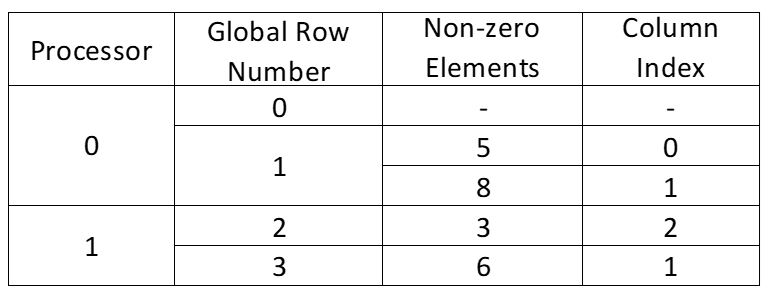
\includegraphics[width=0.4\textwidth]{plots/data.JPG}
	\end{center}
	\caption{Schematic representation of matrix data-structure for each processor}
	\label{fig1} 
\end{figure}
The solution vector \textbf{x} is stored completely on each processors.\\
The most time consuming linear algebra operations in the conjugate gradient algorithm are as follows:
\begin{enumerate}
	\item Matrix-vector multiplication
	\item Scaled Addition of two vectors
	\item Dot product of two vectors	
\end{enumerate}
Theses operations should be parallelized in an efficient way to get the maximum speedup.  The rest of the algorithm can be used unchanged.  
\subsubsection{Matrix-vector Multiplication}\label{mpi}
Matrix-vector multiplication is used to calculate the residual in the conjugate gradient algorithm. Consider a matrix-vector multiplication $\textbf{y}=\textbf{Ax}$. 
\begin{equation*}
\begin{bmatrix}
& & & & & \\
& & & & & \\
& & \mathbf{A}& & & \\
& & & & & \\
& & & & & \\
& & & & & 
\end{bmatrix}
\begin{Bmatrix}
\\
\\
\mathbf{x}\\
\\
\\
\\	
\end{Bmatrix}
= \begin{Bmatrix}
\\
\\
\mathbf{y}\\
\\
\\
\\	
\end{Bmatrix} 
\end{equation*}
The $i$th element in \textbf{y} can be expressed as:
\begin{equation}\label{eq1}
y_i= \textbf{A}_i\textbf{x}=\sum_{k=1}^{n}\textbf{A}_{i,k}\textbf{x}_k
\end{equation}
In CRS data-structure we only store non-zero elements and their corresponding column indices. Hence, the Eq. \ref{eq1} can be expressed as:
\begin{equation}
y_i = \sum_{k=1}^{nnz}\textbf{A}_{i,k}\textbf{x}_{c_k}
\end{equation}
Here, $c_k$ represents the column index for $k$th non-zero element in $i$th row. After parallelization the matrix vector product will be computed on different ranks as
\begin{equation*}
\begin{bmatrix}
\begin{bmatrix}
& & \mathbf{A}_1& & & \\
& & & & & \\
\end{bmatrix}\\
\hline\\
\begin{bmatrix}
& & \mathbf{A}_2& & & \\
& & & & & \\
\end{bmatrix}\\
\hline\\
\begin{bmatrix}
& & \mathbf{A}_3& & & \\
& & & & & \\
\end{bmatrix}\\
\end{bmatrix}
\begin{Bmatrix}
\\
\\
\\
\mathbf{x}\\
\\
\\
\\
\\	
\end{Bmatrix}
=\begin{Bmatrix}
\begin{Bmatrix}
\mathbf{y}_1\\
\\
\end{Bmatrix}\\
\hline\\
\begin{Bmatrix}
\mathbf{y}_2\\
\\
\end{Bmatrix}\\
\hline\\
\begin{Bmatrix}
\mathbf{y}_3\\
\\
\end{Bmatrix}	
\end{Bmatrix} 
\end{equation*}
In the above example, the serial matrix vector product is parallelized with 3 processors. Each processor handles a portion of the matrix  and multiplies it with full vector $\mathbf{x}$ to obtain the portion of the result vector. After the computation is completed by all the processors, all the locally computed elements are sent to all other processors. Better efficiency is achieved if the rows are distributed evenly across the processors.   

\subsubsection{Vector Addition}
Consider an addition of two vectors $\mathbf{x} + \mathbf{y} = \mathbf{z}$ i.e.
\begin{equation*}
\begin{Bmatrix}
\\
\\
\mathbf{x}\\
\\
\\
\\	
\end{Bmatrix} +
\begin{Bmatrix}
\\
\\
\mathbf{y}\\
\\
\\
\\	
\end{Bmatrix}
= \begin{Bmatrix}
\\
\\
\mathbf{z}\\
\\
\\
\\	
\end{Bmatrix}
\end{equation*}
Parallelizing the elementwise operations such as this with multiple processors very straightforward
\begin{equation*}
\begin{Bmatrix}
\begin{Bmatrix}
\mathbf{x}_1\\
\\
\end{Bmatrix}\\
\hline\\
\begin{Bmatrix}
\mathbf{x}_2\\
\\
\end{Bmatrix}\\
\hline\\
\begin{Bmatrix}
\mathbf{x}_3\\
\\
\end{Bmatrix}	
\end{Bmatrix} + 
\begin{Bmatrix}
\begin{Bmatrix}
\mathbf{y}_1\\
\\
\end{Bmatrix}\\
\hline\\
\begin{Bmatrix}
\mathbf{y}_2\\
\\
\end{Bmatrix}\\
\hline\\
\begin{Bmatrix}
\mathbf{y}_3\\
\\
\end{Bmatrix}	
\end{Bmatrix} = 
\begin{Bmatrix}
\begin{Bmatrix}
\mathbf{z}_1\\
\\
\end{Bmatrix}\\
\hline\\
\begin{Bmatrix}
\mathbf{z}_2\\
\\
\end{Bmatrix}\\
\hline\\
\begin{Bmatrix}
\mathbf{z}_3\\
\\
\end{Bmatrix}	
\end{Bmatrix}
\end{equation*}
Each processor will compute the sum of the specific set of rows which it operates on and will store the partial results in a local variable.

\subsubsection{Dot Product}
Dot product operation between two vectors is required for calculation of step size $\alpha$. The dot product between two vectors of size $n$ can be expressed as: $\textbf{x}.\textbf{y}=\sum_{i=1}^{n}\textbf{x}_i\textbf{y}_i$. 
\begin{equation*}
\begin{Bmatrix}
\\
\\
\mathbf{x}\\
\\
\\
\\	
\end{Bmatrix} \cdot
\begin{Bmatrix}
\\
\\
\mathbf{y}\\
\\
\\
\\	
\end{Bmatrix}
= sum\begin{Bmatrix}
\\
\\
\mathbf{x}\circ \mathbf{y}\\
\\
\\
\\	
\end{Bmatrix}
\end{equation*}

Both of the vectors are similarly distributed across the processors. Each processor calculates the partial dot product corresponding to its allocated elements as

\begin{equation*}
\begin{Bmatrix}
\begin{Bmatrix}
\mathbf{x}_1\\
\\
\end{Bmatrix}\\
\hline\\
\begin{Bmatrix}
\mathbf{x}_2\\
\\
\end{Bmatrix}\\
\hline\\
\begin{Bmatrix}
\mathbf{x}_3\\
\\
\end{Bmatrix}	
\end{Bmatrix} \cdot 
\begin{Bmatrix}
\begin{Bmatrix}
\mathbf{y}_1\\
\\
\end{Bmatrix}\\
\hline\\
\begin{Bmatrix}
\mathbf{y}_2\\
\\
\end{Bmatrix}\\
\hline\\
\begin{Bmatrix}
\mathbf{y}_3\\
\\
\end{Bmatrix}	
\end{Bmatrix} = 
sum\begin{Bmatrix}
sum\begin{Bmatrix}
\mathbf{x}_1 \circ \mathbf{y}_1\\
\\
\end{Bmatrix}\\
\hline\\
sum\begin{Bmatrix}
\mathbf{x}_2 \circ \mathbf{y}_2\\
\\
\end{Bmatrix}\\
\hline\\
sum\begin{Bmatrix}
\mathbf{x}_3 \circ \mathbf{y}_3\\
\\
\end{Bmatrix}	
\end{Bmatrix}
\end{equation*}


 The partial dot product for $k$th processor can be expressed as follows:
\begin{equation}
s_k =\sum_{i=f_k}^{l_k}\textbf{x}_i\textbf{y}_i
\end{equation}
Here, $f_k$ and $l_k$ are respectively first and last indices of elements stored on $k$th processors. These partial dot products are  sent to the master processor using MPI\_Send and MPI\_Rec operations. The final dot product for $m$ processors is calculated on the mater processor as follows:
\begin{equation}
\textbf{x}.\textbf{y}= \sum_{k=1}^{m}s_k
\end{equation}
Finally, every processor requires a copy of complete dot product value for further operations. This achieved by MPI broadcast operation (MPI\_Bcast) where dot product value is sent to all the processors from master processor.

\subsection{CUDA Implementation}
\subsection{MPI I/O}
MPI I/O modules are optimally implemented in the algorithm at three instances -- loading all partitioned input data in the right processor, load the full update vector on to each rank (after it is partially updated by each rank) and to write the partial final results from each rank to a common output file.

\subsubsection{Reading Partitioned Inputs}
The following binary files are required as inputs to solve the system of equations
\begin{enumerate}
	\item \texttt{Mvec} -- File which stores the sparse matrix as a vector
	\item \texttt{rowp} -- File storing the auxiliary array pointing to the index of first non-zero element of each row in \texttt{Mvec}
	\item \texttt{colm} -- File storing the column index of all non-zero entries
	\item \texttt{rhs} -- File storing the full RHS vector (i.e. $\mathbf{b}$ in $\mathbf{A}\mathbf{x}=\mathbf{b}$)
\end{enumerate} 

All the processors will have its own copy of the full RHS vector. The other 3 vectors are partitioned and read into each processor to ensure that values corresponding to the set of rows assigned to a processor are only read. 

The routine \texttt{MPI\_File\_read\_at()} is used to ensure that each process reads the right chunk of data from the input files and load them in relevant variables.

\subsubsection{Loading Update Vector}
The algorithm can be realized by using only one full-vector (i.e. a vector that is stored in its entirety on each rank). The update vector $\mathbf{p_k}$ in our programme is the only full-vector as it is the only one involved in the matrix-vector product. On each processor, the partial vector result of the partial matrix full vector product is computed as in fig \ref{fig2}
\begin{figure}[H]
	\begin{center}
		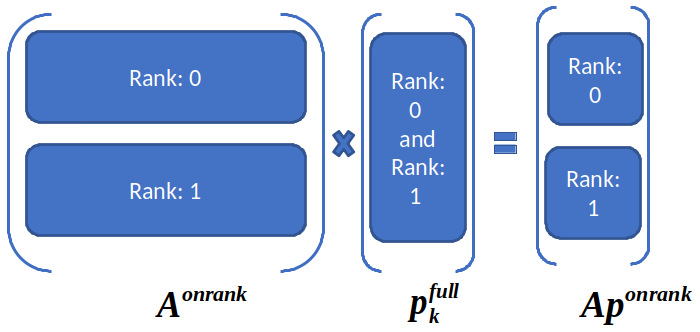
\includegraphics[width=0.5\textwidth]{plots/mpio_Ap.png}
	\end{center}
	\caption{Matrix-vector product on multiple ranks}
	\label{fig2} 
\end{figure}
The subsequent operations operations to get the new update vector $\mathbf{p_{k+1}}$ are done using the scaled vector addition and dot product kernels. The new update vector, however is stored partially on each rank based on the calculations from that rank.
\begin{figure}[H]
	\begin{center}
		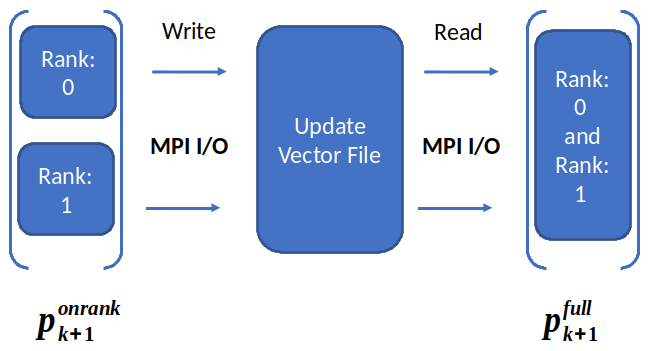
\includegraphics[width=0.5\textwidth]{plots/mpio_pupdate.png}
	\end{center}
	\caption{Partial update vector on each rank to full update vector using MPI I/O}
	\label{fig3} 
\end{figure}

 \texttt{MPI\_File\_write\_at()} routine is used to write the partial update vector on each rank to a common file \texttt{update\_vector}. After all ranks finish writing the update vector to the file, using \texttt{MPI\_File\_read\_all()} the full update vector is read into a variable. Therefore, all ranks will have a copy of the full update vector for the matrix vector multiplication in the next iteration.

\subsubsection{Writing Final Result}
The solution to given linear system i.e. the result vector is also stored in each processor partially. The results were written to output file(s) in two ways -- 
\begin{enumerate}
	\item To one common result file using \texttt{MPI\_File\_write\_at()} ensuring each processor writes the partial result in the right location
	\item To multiple result files (one from each rank) using \texttt{MPI\_File\_write\_all()}
\end{enumerate}
 
\subsection{Template Styles}

The primary parameter given to the ``\verb|acmart|'' document class is
the {\itshape template style} which corresponds to the kind of publication
or SIG publishing the work. This parameter is enclosed in square
brackets and is a part of the {\verb|documentclass|} command:
\begin{verbatim}
  \documentclass[STYLE]{acmart}
\end{verbatim}

Journals use one of three template styles. All but three ACM journals
use the {\verb|acmsmall|} template style:
\begin{itemize}
\item {\verb|acmsmall|}: The default journal template style.
\item {\verb|acmlarge|}: Used by JOCCH and TAP.
\item {\verb|acmtog|}: Used by TOG.
\end{itemize}

The majority of conference proceedings documentation will use the {\verb|acmconf|} template style.
\begin{itemize}
\item {\verb|acmconf|}: The default proceedings template style.
\item{\verb|sigchi|}: Used for SIGCHI conference articles.
\item{\verb|sigchi-a|}: Used for SIGCHI ``Extended Abstract'' articles.
\item{\verb|sigplan|}: Used for SIGPLAN conference articles.
\end{itemize}

\subsection{Template Parameters}

In addition to specifying the {\itshape template style} to be used in
formatting your work, there are a number of {\itshape template parameters}
which modify some part of the applied template style. A complete list
of these parameters can be found in the {\itshape \LaTeX\ User's Guide.}

Frequently-used parameters, or combinations of parameters, include:
\begin{itemize}
\item {\verb|anonymous,review|}: Suitable for a ``double-blind''
  conference submission. Anonymizes the work and includes line
  numbers. Use with the \verb|\acmSubmissionID| command to print the
  submission's unique ID on each page of the work.
\item{\verb|authorversion|}: Produces a version of the work suitable
  for posting by the author.
\item{\verb|screen|}: Produces colored hyperlinks.
\end{itemize}

This document uses the following string as the first command in the
source file:
\begin{verbatim}
\documentclass[sigplan,screen]{acmart}
\end{verbatim}

\section{Modifications}

Modifying the template --- including but not limited to: adjusting
margins, typeface sizes, line spacing, paragraph and list definitions,
and the use of the \verb|\vspace| command to manually adjust the
vertical spacing between elements of your work --- is not allowed.

{\bfseries Your document will be returned to you for revision if
  modifications are discovered.}

\section{Typefaces}

The ``\verb|acmart|'' document class requires the use of the
``Libertine'' typeface family. Your \TeX\ installation should include
this set of packages. Please do not substitute other typefaces. The
``\verb|lmodern|'' and ``\verb|ltimes|'' packages should not be used,
as they will override the built-in typeface families.

\section{Title Information}

The title of your work should use capital letters appropriately -
\url{https://capitalizemytitle.com/} has useful rules for
capitalization. Use the {\verb|title|} command to define the title of
your work. If your work has a subtitle, define it with the
{\verb|subtitle|} command.  Do not insert line breaks in your title.

If your title is lengthy, you must define a short version to be used
in the page headers, to prevent overlapping text. The \verb|title|
command has a ``short title'' parameter:
\begin{verbatim}
  \title[short title]{full title}
\end{verbatim}

\section{Authors and Affiliations}

Each author must be defined separately for accurate metadata
identification. Multiple authors may share one affiliation. Authors'
names should not be abbreviated; use full first names wherever
possible. Include authors' e-mail addresses whenever possible.

Grouping authors' names or e-mail addresses, or providing an ``e-mail
alias,'' as shown below, is not acceptable:
\begin{verbatim}
  \author{Brooke Aster, David Mehldau}
  \email{dave,judy,steve@university.edu}
  \email{firstname.lastname@phillips.org}
\end{verbatim}

The \verb|authornote| and \verb|authornotemark| commands allow a note
to apply to multiple authors --- for example, if the first two authors
of an article contributed equally to the work.

If your author list is lengthy, you must define a shortened version of
the list of authors to be used in the page headers, to prevent
overlapping text. The following command should be placed just after
the last \verb|\author{}| definition:
\begin{verbatim}
  \renewcommand{\shortauthors}{McCartney, et al.}
\end{verbatim}
Omitting this command will force the use of a concatenated list of all
of the authors' names, which may result in overlapping text in the
page headers.

The article template's documentation, available at
\url{https://www.acm.org/publications/proceedings-template}, has a
complete explanation of these commands and tips for their effective
use.

Note that authors' addresses are mandatory for journal articles.

\section{Rights Information}

Authors of any work published by ACM will need to complete a rights
form. Depending on the kind of work, and the rights management choice
made by the author, this may be copyright transfer, permission,
license, or an OA (open access) agreement.

Regardless of the rights management choice, the author will receive a
copy of the completed rights form once it has been submitted. This
form contains \LaTeX\ commands that must be copied into the source
document. When the document source is compiled, these commands and
their parameters add formatted text to several areas of the final
document:
\begin{itemize}
\item the ``ACM Reference Format'' text on the first page.
\item the ``rights management'' text on the first page.
\item the conference information in the page header(s).
\end{itemize}

Rights information is unique to the work; if you are preparing several
works for an event, make sure to use the correct set of commands with
each of the works.

The ACM Reference Format text is required for all articles over one
page in length, and is optional for one-page articles (abstracts).

\section{CCS Concepts and User-Defined Keywords}

Two elements of the ``acmart'' document class provide powerful
taxonomic tools for you to help readers find your work in an online
search.

The ACM Computing Classification System ---
\url{https://www.acm.org/publications/class-2012} --- is a set of
classifiers and concepts that describe the computing
discipline. Authors can select entries from this classification
system, via \url{https://dl.acm.org/ccs/ccs.cfm}, and generate the
commands to be included in the \LaTeX\ source.

User-defined keywords are a comma-separated list of words and phrases
of the authors' choosing, providing a more flexible way of describing
the research being presented.

CCS concepts and user-defined keywords are required for for all
articles over two pages in length, and are optional for one- and
two-page articles (or abstracts).

\section{Sectioning Commands}



\section{Tables}

The ``\verb|acmart|'' document class includes the ``\verb|booktabs|''
package --- \url{https://ctan.org/pkg/booktabs} --- for preparing
high-quality tables.

Table captions are placed {\itshape above} the table.

Because tables cannot be split across pages, the best placement for
them is typically the top of the page nearest their initial cite.  To
ensure this proper ``floating'' placement of tables, use the
environment \textbf{table} to enclose the table's contents and the
table caption.  The contents of the table itself must go in the
\textbf{tabular} environment, to be aligned properly in rows and
columns, with the desired horizontal and vertical rules.  Again,
detailed instructions on \textbf{tabular} material are found in the
\textit{\LaTeX\ User's Guide}.

Immediately following this sentence is the point at which
Table~\ref{tab:freq} is included in the input file; compare the
placement of the table here with the table in the printed output of
this document.

\begin{table}[H]
  \caption{Frequency of Special Characters}
  \label{tab:freq}
  \begin{tabular}{ccl}
    Non-English or Math&Frequency&Comments\\
    \O & 1 in 1,000& For Swedish names\\
    $\pi$ & 1 in 5& Common in math\\
    \$ & 4 in 5 & Used in business\\
    $\Psi^2_1$ & 1 in 40,000& Unexplained usage\\
\end{tabular}
\end{table}

To set a wider table, which takes up the whole width of the page's
live area, use the environment \textbf{table*} to enclose the table's
contents and the table caption.  As with a single-column table, this
wide table will ``float'' to a location deemed more
desirable. Immediately following this sentence is the point at which
Table~\ref{tab:commands} is included in the input file; again, it is
instructive to compare the placement of the table here with the table
in the printed output of this document.

\section{Math Equations}
You may want to display math equations in three distinct styles:
inline, numbered or non-numbered display.  Each of the three are
discussed in the next sections.

\subsection{Inline (In-text) Equations}
A formula that appears in the running text is called an inline or
in-text formula.  It is produced by the \textbf{math} environment,
which can be invoked with the usual
\texttt{{\char'134}begin\,\ldots{\char'134}end} construction or with
the short form \texttt{\$\,\ldots\$}. You can use any of the symbols
and structures, from $\alpha$ to $\omega$, available in
\LaTeX~\cite{Lamport:LaTeX}; this section will simply show a few
examples of in-text equations in context. Notice how this equation:
\begin{math}
  \lim_{n\rightarrow \infty}x=0
\end{math},
set here in in-line math style, looks slightly different when
set in display style.  (See next section).

\subsection{Display Equations}
A numbered display equation---one set off by vertical space from the
text and centered horizontally---is produced by the \textbf{equation}
environment. An unnumbered display equation is produced by the
\textbf{displaymath} environment.

Again, in either environment, you can use any of the symbols and
structures available in \LaTeX\@; this section will just give a couple
of examples of display equations in context.  First, consider the
equation, shown as an inline equation above:
\begin{equation}
  \lim_{n\rightarrow \infty}x=0
\end{equation}
Notice how it is formatted somewhat differently in
the \textbf{displaymath}
environment.  Now, we'll enter an unnumbered equation:
\begin{displaymath}
  \sum_{i=0}^{\infty} x + 1
\end{displaymath}
and follow it with another numbered equation:
\begin{equation}
  \sum_{i=0}^{\infty}x_i=\int_{0}^{\pi+2} f
\end{equation}
just to demonstrate \LaTeX's able handling of numbering.

\section{Figures}

Your figures should contain a caption which describes the figure to
the reader. Figure captions go below the figure. Your figures should
{\bfseries also} include a description suitable for screen readers, to
assist the visually-challenged to better understand your work.

Figure captions are placed {\itshape below} the figure.

\subsection{The ``Teaser Figure''}

A ``teaser figure'' is an image, or set of images in one figure, that
are placed after all author and affiliation information, and before
the body of the article, spanning the page. If you wish to have such a
figure in your article, place the command immediately before the
\verb|\maketitle| command:
\begin{verbatim}
  \begin{teaserfigure}
    \includegraphics[width=\textwidth]{sampleteaser}
    \caption{figure caption}
  \end{teaserfigure}
\end{verbatim}

\section{Citations and Bibliographies}

The use of \BibTeX\ for the preparation and formatting of one's
references is strongly recommended. Authors' names should be complete
--- use full first names (``Donald E. Knuth'') not initials
(``D. E. Knuth'') --- and the salient identifying features of a
reference should be included: title, year, volume, number, pages,
article DOI, etc.

The bibliography is included in your source document with these two
commands, placed just before the \verb|\end{document}| command:
\begin{verbatim}
  \bibliographystyle{ACM-Reference-Format}
  \bibliography{bibfile}
\end{verbatim}
where ``\verb|bibfile|'' is the name, without the ``\verb|.bib|''
suffix, of the \BibTeX\ file.

Citations and references are numbered by default. A small number of
ACM publications have citations and references formatted in the
``author year'' style; for these exceptions, please include this
command in the {\bfseries preamble} (before the command
``\verb|\begin{document}|'') of your \LaTeX\ source:
\begin{verbatim}
  \citestyle{acmauthoryear}
\end{verbatim}

  Some examples.  A paginated journal article \cite{Abril07}, like this.

%% The next two lines define the bibliography style to be used, and
%% the bibliography file.
\bibliographystyle{ACM-Reference-Format}
\bibliography{acmart}

%%
%% If your work has an appendix, this is the place to put it.
\appendix

\end{document}
\endinput
%%
%% End of file `sample-sigplan.tex'.
